\part{Personagem Principal - Veículo}

\section{Descrição}

	O personagem principal do jogo será basicamente o carro utilizado, nunca será visto um piloto então não haverá simulações de personagens humanos.

\begin{figure}[!h]
		\centering
	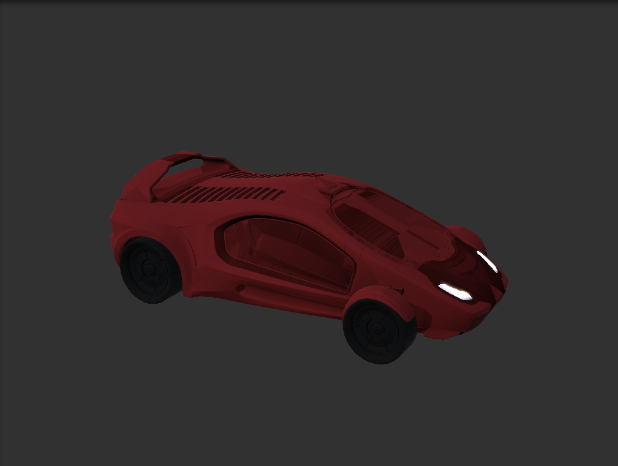
\includegraphics[scale=0.5]{figuras/carro}
		\caption{Imagem do carro de jogo}
\end{figure}
	
\section{Atributos}

	\begin{enumerate}
	
		\item O carro será construido tomando como base o ambiente externo ao percurso, procurando ser realista com base nas proporções do mundo real. 
		\item A movimentação será medida com base no medidor em barras.
		\item Haverá coleta de itens para pontuação, onde acontecerá ao primeiro contato com o carro.
		\item Não haverá danos, onde o carro batendo ou saindo da pista, a corrida encerra.
		\item Comandos para o carro: \hyperlink{teclas}{link}
		\item O carro pode andar apenas dentro da pista
	
	\end{enumerate}